\documentclass{article}
\usepackage{amsmath}
\usepackage{amssymb}
\usepackage{graphicx}
\usepackage{hyperref}
\usepackage[version=4]{mhchem}

\title{Example 7}
\date{}

\begin{document}
\maketitle

In the figure \(X O=8, Z O=6\), and the vertex \(Y\) of rectangle \(X Y Z O\) lies on circle \(O\). Find the area of the shaded region. Express your answer in terms of \(\pi\).

Solution: \(25 \pi-48\) (units \({ }^{2}\) )\\
Connect \(Y O\). We see that triangle \(O X Y\) is a 6-8-10 right\\
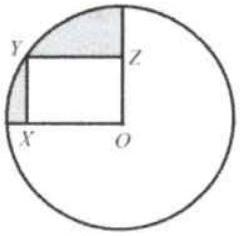
\includegraphics[width=\textwidth]{images/problem_image_1.jpg} triangle. So the radius of the circle is 10 . The area of the circle is \(\pi \times 10^{2}=100 \pi\). The area of the quarter circle is \(25 \pi\). The shaded area is \(25 \pi-6 \times 8=25 \pi-48\)\\
\centering
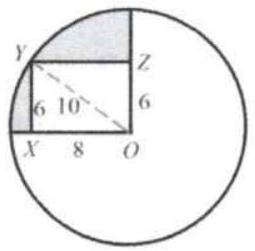
\includegraphics[width=\textwidth]{images/reasoning_image_1.jpg}


\end{document}
